\documentclass{article}
\usepackage{graphicx} % Required for inserting images
\usepackage{fancyhdr} % Header
\usepackage{lastpage}
\usepackage[a4paper, total={6in, 8in}]{geometry}
\usepackage{float} % Floating position
\usepackage{hyperref} % Links
\usepackage{amsmath} % Math
\usepackage{amssymb} % Math
\usepackage{listings} % Import code in appendix
\usepackage{xcolor} % For coloring code
% Listing Configuration
\lstset{
    language=Python,
    basicstyle=\ttfamily\small,
    keywordstyle=\color{blue},
    stringstyle=\color{red},
    commentstyle=\color{green},
    showstringspaces=false,
    breaklines=true,
    frame=single
}
\usepackage{tikz} % Graph
\usetikzlibrary{bayesnet}
\usetikzlibrary{positioning}
\usetikzlibrary{decorations.markings}

\graphicspath{{images/}}

\newcommand{\authorFst}{Tristan Perrot}
\newcommand{\emailFst}{\href{mailto:tristanp@kth.se}{tristanp@kth.se}}
\newcommand{\authorSnd}{Étienne Riguet}
\newcommand{\emailSnd}{\href{mailto:riguet@kth.se}{riguet@kth.se}}
\newcommand{\authorTrd}{Romain Darous}
\newcommand{\emailTrd}{\href{mailto:darous@kth.se}{darous@kth.se}}
\newcommand{\authorFrth}{Anthony Jones}
\newcommand{\emailFrth}{\href{mailto:arjjones@kth.se}{arjjones@kth.se}}

\pagestyle{fancy}
\fancyhf{} % clear all header and footer fields
\lhead{Large Project Variational Inference \\ DD2434 - Machine Learning, Advanced Course}
\rhead{\authorFst \\ \authorSnd \\ \authorTrd \\ \authorFrth}
\cfoot{\thepage \  / \pageref{LastPage}}
\setlength{\headheight}{47pt}
\setlength{\footskip}{70pt}
\addtolength{\topmargin}{-14pt}

\title{DD2434 - Machine Learning, Advanced Course \\ Project 1.5 - Variational Inference}
\author{\authorFst \\ \emailFst \and \authorSnd \\ \emailSnd \and \authorTrd \\ \emailTrd \and \authorFrth \\ \emailFrth}
\date{December 2023}

\begin{document}

\maketitle

\begin{center}
    
\includegraphics[scale=0.5]{KTH_logo_RGB_bla.png}
\end{center}

\thispagestyle{empty}

\newpage
\tableofcontents
\newpage

\section{Example}

\begin{figure}[H]
    \centering
    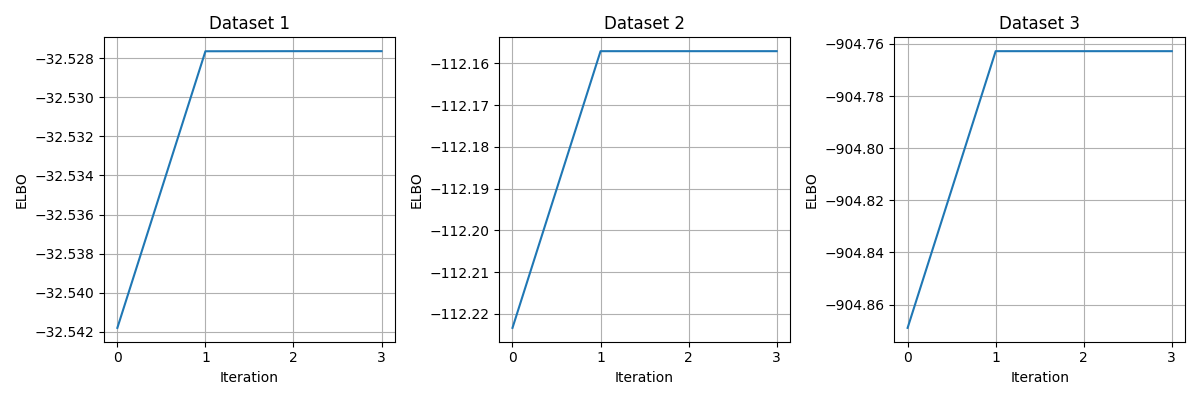
\includegraphics[scale=0.5]{images/15_elbo.png}
    \caption{ELBO plot by datasets}
    \label{fig:3.15.2}
\end{figure}

\newpage
\appendix
\section{Appendix}
\subsection{Question 3.12}\label{appendix:code.3.12}
\lstinputlisting[label = {alg:3.12}]{py_files/3.12.py}

\end{document}